\section{Cálculo de parámetros}

\subsection{Velocidad}

Primero se tiene que conocer la velocidad en cada instante del movimiento.

Para eso se cálcula cada velocidad utilizando la expresión $v = \frac{\Delta x}{\Delta t}$

\clearpage
\begin{longtable}{|c|c|c|c|c|c|c|}
    \hline
    \rowcolor{azulito} & \multicolumn{2}{c|}{Cono 1} & \multicolumn{2}{c|}{Cono 2} & \multicolumn{2}{c|}{Cono 3} \\
    \hline
    \rowcolor{azulito} t(s) & v (m/s) & $\delta v$ & v (m/s) & $\delta v$ & v (m/s) & $\delta v$ \\
    \endhead
    \hline 0.00 & 0.000 & 0.0000 & 0.000 & 0.0000 & 0.000 & 0.0000 \\
    \hline 0.03 & -0.182 & 0.4997 & -0.455 & 0.4993 & -0.061 & 0.4999 \\
    \hline 0.07 & -0.515 & 0.2460 & -0.224 & 0.2459 & -0.104 & 0.2462 \\
    \hline 0.10 & -0.636 & 0.1648 & -0.290 & 0.1647 & -0.200 & 0.1649 \\
    \hline 0.13 & -0.727 & 0.1239 & -0.143 & 0.1238 & -0.218 & 0.1239 \\
    \hline 0.17 & -0.758 & 0.0986 & -0.186 & 0.0986 & -0.210 & 0.0986 \\
    \hline 0.20 & -0.848 & 0.0823 & -0.170 & 0.0823 & -0.170 & 0.0823 \\
    \hline 0.23 & -0.879 & 0.0707 & -0.167 & 0.0706 & -0.167 & 0.0707 \\
    \hline 0.27 & -0.970 & 0.0617 & -0.127 & 0.0616 & -0.157 & 0.0617 \\
    \hline 0.30 & -0.909 & 0.0549 & -0.147 & 0.0549 & -0.153 & 0.0549 \\
    \hline 0.33 & -1.000 & 0.0494 & -0.120 & 0.0494 & -0.144 & 0.0494 \\
    \hline 0.37 & -1.061 & 0.0449 & -0.120 & 0.0448 & -0.112 & 0.0448 \\
    \hline 0.40 & -1.182 & 0.0412 & -0.113 & 0.0411 & -0.118 & 0.0411 \\
    \hline 0.43 & -1.273 & 0.0380 & -0.099 & 0.0380 & -0.122 & 0.0380 \\
    \hline 0.47 & -1.273 & 0.0352 & -0.099 & 0.0352 & -0.124 & 0.0352 \\
    \hline 0.50 & -1.333 & 0.0329 & -0.096 & 0.0329 & -0.118 & 0.0329 \\
    \hline 0.53 & -1.394 & 0.0309 & -0.084 & 0.0309 & -0.113 & 0.0308 \\
    \hline 0.57 & -1.182 & 0.0290 & -0.078 & 0.0290 & -0.104 & 0.0290 \\
    \hline 0.60 & -1.182 & 0.0274 & -0.073 & 0.0274 & -0.098 & 0.0274 \\
    \hline 0.63 & -1.182 & 0.0260 & -0.070 & 0.0260 & -0.100 & 0.0260 \\
    \hline 0.67 & -1.152 & 0.0247 & -0.067 & 0.0247 & -0.082 & 0.0246 \\
    \hline 0.70 & -1.182 & 0.0235 & -0.070 & 0.0235 & -0.080 & 0.0235 \\
    \hline 0.73 & -1.242 & 0.0224 & -0.067 & 0.0224 & -0.076 & 0.0224 \\
    \hline 0.77 & -1.273 & 0.0214 & -0.064 & 0.0214 & -0.073 & 0.0214 \\
    \hline 0.80 & -1.364 & 0.0206 & -0.061 & 0.0206 & -0.073 & 0.0205 \\
    \hline 0.83 & -1.394 & 0.0197 & -0.071 & 0.0197 & -0.071 & 0.0197 \\
    \hline 0.87 & -1.333 & 0.0190 & -0.069 & 0.0190 & -0.068 & 0.0190 \\
    \hline 0.90 & -1.333 & 0.0183 & -0.059 & 0.0183 & -0.064 & 0.0183 \\
    \hline 0.93 & -1.212 & 0.0176 & -0.054 & 0.0176 & -0.062 & 0.0176 \\
    \hline 0.97 & -1.212 & 0.0170 & -0.051 & 0.0170 & -0.054 & 0.0170 \\
    \hline 1.00 & -1.182 & 0.0164 & -0.087 & 0.0164 & -0.057 & 0.0164 \\
    \hline 1.03 & -1.636 & 0.0159 & -0.015 & 0.0159 & -0.054 & 0.0159 \\
    \hline 1.07 & -1.485 & 0.0154 & -0.046 & 0.0154 & -0.054 & 0.0154 \\
    \hline 1.10 & -1.485 & 0.0149 & -0.045 & 0.0149 & -0.050 & 0.0149 \\
    \hline 1.13 & -1.485 & 0.0145 & -0.044 & 0.0145 & -0.050 & 0.0145 \\
    \hline 1.17 & -1.485 & 0.0141 & -0.045 & 0.0141 & -0.047 & 0.0141 \\
    \hline 1.20 & -1.182 & 0.0137 & -0.042 & 0.0137 & -0.047 & 0.0137 \\
    \hline 1.23 & -1.212 & 0.0133 & -0.040 & 0.0133 & -0.044 & 0.0133 \\
    \hline 1.27 & -1.636 & 0.0130 & -0.039 & 0.0130 & -0.044 & 0.0130 \\
    \hline 1.30 & -1.485 & 0.0126 & -0.038 & 0.0126 & -0.043 & 0.0126 \\
    \hline 1.33 & -1.182 & 0.0123 & -0.037 & 0.0123 & -0.041 & 0.0123 \\
    \hline 1.37 & -1.333 & 0.0120 & -0.037 & 0.0120 & -0.040 & 0.0120 \\
    \hline 1.40 & -1.424 & 0.0117 & -0.035 & 0.0117 & -0.039 & 0.0117 \\
    \hline 1.43 & -1.455 & 0.0115 & -0.034 & 0.0115 & -0.037 & 0.0115 \\
    \hline 1.47 & -1.515 & 0.0112 & -0.033 & 0.0112 & -0.035 & 0.0112 \\
    \hline 1.50 & -1.576 & 0.0110 & -0.030 & 0.0110 & -0.041 & 0.0109 \\
    \hline 1.53 & -1.636 & 0.0107 & -0.032 & 0.0107 & -0.002 & 0.0107 \\
    \hline 1.57 & -1.485 & 0.0105 & -0.031 & 0.0105 & 0.0105 & \\
    \hline 1.60 & -1.061 & 0.0103 & -0.028 & & & \\
    \hline 1.63 & -1.485 & 0.0101 & -0.027 & & & \\
    \hline 1.67 & -1.364 & 0.0099 & -0.027 & & & \\
    \hline 1.70 & -1.182 & 0.0097 & -0.023 & & & \\
    \hline 1.73 & -1.182 & 0.0095 &        &        &        & \\
    \hline 1.77 & -1.212 & 0.0093 &        &        &        & \\
    \hline 1.80 & -1.182 & 0.0091 &        &        &        & \\
    \hline 1.83 & -1.273 & 0.0090 &        &        &        & \\
    \hline
    \caption{Velocidades de cada cono calculadas a partir
    de su posición.}
    \label{tab:Vel_Pos}
\end{longtable}
\subsection{Fuerza}

Para poder conocer la fuerza de resistencia que presenta el
aire al cono, obtenemos los valores de la velocidad en cada instante
de tiempo dado.

\begin{figure}[h!]
    \centering
    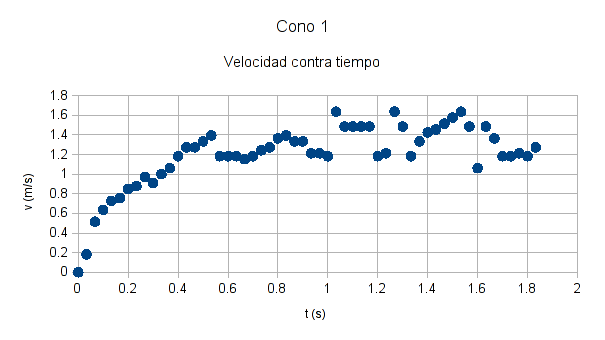
\includegraphics{vel_cono1}
    \caption{La grafica de la velocidad contra tiempo muestra que la velocidad terminal
    fue alcanzada a partir del tiempo 0.567 s y que los valores a partir de este
    tiempo se encuentran en nuestro rango de incertidumbre. Esto nos indica que el
    cono alcanzo su velocidad terminal en ese tiempo.}
    \label{fig:VelCono1}
\end{figure}

\begin{figure}[h!]
    \centering
    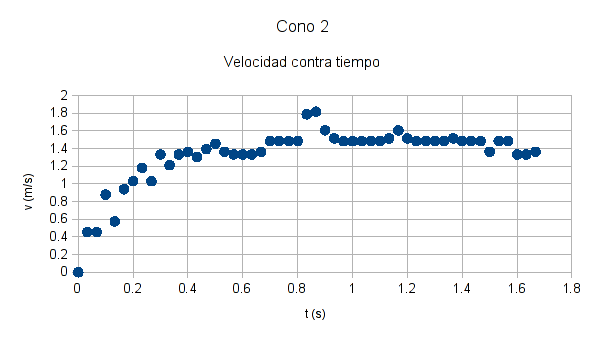
\includegraphics{vel_cono2}j
    \caption{Se observa que llegado el tiempo 0.667 s los valores de velocidad se encuentran
    dentro del rango de incertidumbre, esto nos permite concluir que 
    el cono alcanza su velocidad terminal.}
    \label{fig:VelCono2}
\end{figure}

\begin{figure}[h!]
    \centering
    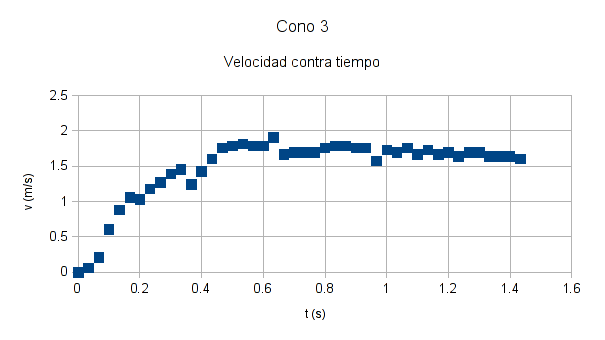
\includegraphics{vel_cono3}
    \caption{Grafica de la velocidad contra tiempo del cono 3 en la que observamos que 
    pasado un tiempo 0.700 s su velocidad se encuentra en un rango que se encuentra contenido
    dentro de las incertidumbres calculadas mostrando que alcanzo su velocidad terminal.}
    \label{fig:VelCono3}
\end{figure}
\subsection{Valor de $r$}

Ajustamos un recta a los valores graficados en
\ref{fig:posl_cono1}, \ref{fig:pos1_cono2} y \ref{fig:pos1_cono3}.
con la pendiente de dichas rectas obtenemos la velocidad
terminal de cada cono, así sustituyendo en las ecuaciones
\ref{int_valorDeR}.

\begin{table}
    \centering
    \begin{tabular}{|c|c|}
        \hline
        \rowcolor{azulito} Cono & Velocidad Terminal (m/s) \\
%         \hline 1 & -1.27384 \\
%         \hline 2 & -1.42074 \\
%         \hline 3 & -1.60727 \\
        \hline 1 & -1.273 \\
        \hline 2 & -1.420 \\
        \hline 3 & -1.607 \\
        \hline
    \end{tabular}
    \caption{En esta tabla se muestran los valores
    de la pendiente de la recta ajustada a los datos
    obtenidos en las tablas \ref{tab:postiemcono}.}
    \label{tab:VelTerminal}
\end{table}

Una vez conocidos las velocidades terminales de cada uno de los
conos, vamos a buscar conocer un valor de $r$ que nos permita
igualar la fuerza de atracción gravitacional con una fuerza que 
sea proporcional al cuadrado de la velocidad.

Se propone un valor para $r$ de 0.0095 y se multiplica este
valor por $v^2$ y se compara con la fuerza gravitacional que
sufre el cono.
\subsection{Valor de $C_D$}

Ya con el valor de $r$ bien definido, podemos conocer el
$C_D$, con la expresión \ref{int_valorDeR}:

Pero antes debemos calcular el área de los conos, para eso
hacemos uso de las expresiones \ref{AreaCono}, \ref{Perimetro}
y \ref{Arco}.

$\frac{31 \pi}{18}(0.1 m) = 2\pi R$
entonces $R = \frac{31}{360} \approx 0.086 m$

Y ahora si podemos obtener el área:

$A = \pi (0.086 m) (0.1 m) = \pi \frac{31}{3600} \approx 0.027m^2$

Entonces nuestro valor de $C_D$ es:

$ = \frac{2r}{\rho A} = \frac{2(0.0105\frac{kg}{m}}{1\frac{kg}{m^3}(0.027 m^2}) \approx 0.776$
